\documentclass[journal,12pt,twocolumn]{IEEEtran}
\usepackage{amsthm}
\usepackage{gensymb}
\usepackage{setspace}
\singlespacing
\usepackage[cmex10]{amsmath}
\usepackage{bm}

\usepackage{cases}
\usepackage{mathrsfs}
\usepackage{cite}
\usepackage{stfloats}
\usepackage{mathtools}
\usepackage[breaklinks=true]{hyperref}
\usepackage{graphicx}
\usepackage{subfig}
\usepackage{txfonts}
\usepackage{longtable}
\usepackage{multirow}
\usepackage{tfrupee}
\usepackage{enumitem}
\usepackage{tikz}
\usepackage{steinmetz}
\usepackage{verbatim}
\usepackage{circuitikz}
\usepackage{tkz-euclide}





\usetikzlibrary{calc,math}
\usepackage{listings}
    \usepackage{color}                                            %%
    \usepackage{array}                                            %%
    \usepackage{longtable}                                        %%
    \usepackage{calc}                                             %%
    \usepackage{multirow}                                         %%
    \usepackage{hhline}                                           %%
    \usepackage{ifthen}                                           %%
    \usepackage{lscape}     
\usepackage{multicol}
\usepackage{chngcntr}

\DeclareMathOperator*{\Res}{Res}

\renewcommand\thesection{\arabic{section}}
\renewcommand\thesubsection{\thesection.\arabic{subsection}}
\renewcommand\thesubsubsection{\thesubsection.\arabic{subsubsection}}

\renewcommand \thesectiondis{\arabic{section}}
\renewcommand\thesubsectiondis{\thesectiondis.\arabic{subsection}}
\renewcommand\thesubsubsectiondis{\thesubsectiondis.\arabic{subsubsection}}


\hyphenation{op-tical net-works semi-conduc-tor}
\def\inputGnumericTable{}                                 %%

\lstset{
%language=C,
frame=single, 
breaklines=true,
columns=fullflexible
}
\begin{document}

\newcommand{\BEQA}{\begin{eqnarray}}
\newcommand{\EEQA}{\end{eqnarray}}
\newcommand{\define}{\stackrel{\triangle}{=}}
\bibliographystyle{IEEEtran}
\raggedbottom
\setlength{\parindent}{0pt}
\providecommand{\mbf}{\mathbf}
\providecommand{\pr}[1]{\ensuremath{\Pr\left(#1\right)}}
\providecommand{\qfunc}[1]{\ensuremath{Q\left(#1\right)}}
\providecommand{\sbrak}[1]{\ensuremath{{}\left[#1\right]}}
\providecommand{\lsbrak}[1]{\ensuremath{{}\left[#1\right.}}
\providecommand{\rsbrak}[1]{\ensuremath{{}\left.#1\right]}}
\providecommand{\brak}[1]{\ensuremath{\left(#1\right)}}
\providecommand{\lbrak}[1]{\ensuremath{\left(#1\right.}}
\providecommand{\rbrak}[1]{\ensuremath{\left.#1\right)}}
\providecommand{\cbrak}[1]{\ensuremath{\left\{#1\right\}}}
\providecommand{\lcbrak}[1]{\ensuremath{\left\{#1\right.}}
\providecommand{\rcbrak}[1]{\ensuremath{\left.#1\right\}}}
\theoremstyle{remark}
\newtheorem{rem}{Remark}
\newcommand{\sgn}{\mathop{\mathrm{sgn}}}
\providecommand{\abs}[1]{\vert#1\vert}
\providecommand{\res}[1]{\Res\displaylimits_{#1}} 
\providecommand{\norm}[1]{\lVert#1\rVert}
%\providecommand{\norm}[1]{\lVert#1\rVert}
\providecommand{\mtx}[1]{\mathbf{#1}}
\providecommand{\mean}[1]{E[ #1 ]}
\providecommand{\fourier}{\overset{\mathcal{F}}{ \rightleftharpoons}}
%\providecommand{\hilbert}{\overset{\mathcal{H}}{ \rightleftharpoons}}
\providecommand{\system}{\overset{\mathcal{H}}{ \longleftrightarrow}}
	%\newcommand{\solution}[2]{\textbf{Solution:}{#1}}
\newcommand{\solution}{\noindent \textbf{Solution: }}
\newcommand{\cosec}{\,\text{cosec}\,}
\providecommand{\dec}[2]{\ensuremath{\overset{#1}{\underset{#2}{\gtrless}}}}
\newcommand{\myvec}[1]{\ensuremath{\begin{pmatrix}#1\end{pmatrix}}}
\newcommand{\mydet}[1]{\ensuremath{\begin{vmatrix}#1\end{vmatrix}}}
\numberwithin{equation}{subsection}
\makeatletter
\@addtoreset{figure}{problem}
\makeatother
\let\StandardTheFigure\thefigure
\let\vec\mathbf
\renewcommand{\thefigure}{\theproblem}
\def\putbox#1#2#3{\makebox[0in][l]{\makebox[#1][l]{}\raisebox{\baselineskip}[0in][0in]{\raisebox{#2}[0in][0in]{#3}}}}
     \def\rightbox#1{\makebox[0in][r]{#1}}
     \def\centbox#1{\makebox[0in]{#1}}
     \def\topbox#1{\raisebox{-\baselineskip}[0in][0in]{#1}}
     \def\midbox#1{\raisebox{-0.5\baselineskip}[0in][0in]{#1}}
\vspace{3cm}
\title{Assignment6}%number
\author{CS20Btech11035 -NYALAPOGULA MANASWINI}
\maketitle
\newpage
\bigskip

\renewcommand{\thefigure}{\theenumi}
\renewcommand{\thetable}{\theenumi}
Download python code from 
\begin{lstlisting}
https://github.com/N-Manaswini23/assignment6/blob/main/python%20codes/assignment6.py
\end{lstlisting}
%
Download latex code from 
\begin{lstlisting}
https://github.com/N-Manaswini23/assignment6/blob/main/assignment6.tex
\end{lstlisting}
%

\section*{GATE 2019 ME set-2 QUESTION 28}
The variable $x$ takes a value between $0$ and $10$ with uniform probability distribution. The variable $y$ takes a value between $0$ and $20$ with uniform probability distribution.The probability that sum of variables $(x+y)$ being greater than $20$ is

\section*{SOLUTION}
Let $X$ and $Y$ be two independent random variables. \\
Let $Z$ be another random variable where $Z=X+Y$
$X \in \sbrak{0,10}$,$Y \in \sbrak{0,20}$,$Z \in \sbrak{0,30}$
\begin{align}
\int_{0}^{10} p_X(x) \mathrm{dx} &=1  \\
\therefore p_X(x)&=\frac{1}{10} \label{px}
\end{align}
The PDF for $X$ is
\begin{align}
p_X(x)  = 
\begin{cases}
     \frac{1}{10} & 0 \leq x \leq 10\\
     0 & otherwise \label{1}
\end{cases}
\end{align}
Similarly,PDF for $Y$ is
\begin{align}
p_{Y}(y)  = 
\begin{cases}
     \frac{1}{20} & 0 \leq y \leq 20 \\
      0 & otherwise \label{2}
\end{cases}
\end{align}
$x=z-y$.Using this pdf of X can be written as
\begin{align}
p_X(z-y)  = 
\begin{cases}
    \frac{1}{10} & 0 \leq z-y \leq 10\\
    0 & otherwise \label{3}
\end{cases}
\end{align}
\begin{align}
   z-10 &\leq y \leq z \label{4} \\
   0 &\leq y \leq 20 \label{5}
\end{align}
pdf of $Z$ by convolution can be written as
\begin{align}
 p_Z(z) =  \int_{- \infty}^{\infty} p_X(z-y)p_Y(y) \mathrm{dy} \label{pz}
\end{align}
From \ref{2} and \ref{3}
\begin{align}
 p_Z(z) = \frac{1}{200} \int_{- \infty}^{\infty} \mathrm{dy} \label{6}
\end{align}
For $0 \leq z \leq 10$  
\begin{align}
p_Z(z) &= \frac{1}{200}  \int_{0}^{z}\mathrm{dy}  \\
       &= \frac{z}{200} \label{7}
\end{align}
For $ 10 < z \leq 20 $,
\begin{align}
p_Z(z) &= \frac{1}{200}  \int_{z-10}^{z}\mathrm{dy}  \\
        &= \frac{1}{20} \label{8}
\end{align}
For $ 20 < z \leq 30 $,
\begin{align}
p_Z(z) &=\frac{1}{200}  \int_{z-10}^{20}\mathrm{dy}  \\
       &= \frac{30-z}{200} \label{9}
\end{align}
$\therefore$ PDF of $Z$ is as follows
\begin{align}
p_{Z}(z)  = 
\begin{cases}
  \frac{z}{200}& 0 \leq z \leq 10 \\
  \frac{1}{20} & 10 < z \leq 20 \\
  \frac{30-z}{200} & 20 < z \leq 30 \\
  0 & otherwise \label{10}
\end{cases}
\end{align}
\begin{equation}
F_Z(z) = \Pr(Z \leq z) \label{cdf}
\end{equation}
The CDF  of $Z$ is as follows:
\begin{align}
F_Z(z)  = 
\begin{cases}
0 & z < 0 \\
  \frac{z^2}{400} &  z \leq 10 \\
  \frac{z-5}{20} &  z \leq 20 \\
  \frac{60z -500 -z^2}{400} & z \leq 30 \\
  1 & z > 30 \label{11}
\end{cases}
\end{align}
\begin{align}
\Pr(z > 20)&= 1- F_Z(20) \\
           &=\frac{1}{4} \label{12} \\
\therefore \Pr(x+y>20)&=\frac{1}{4}=0.25
\end{align}
\begin{figure}[htb!]
\begin{center}
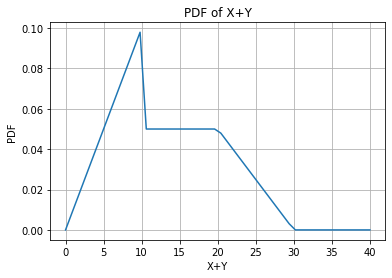
\includegraphics[width=0.5\textwidth]{assignment6pdf.png}
\end{center}
\end{figure}

\begin{figure}[htb!]
\begin{center}
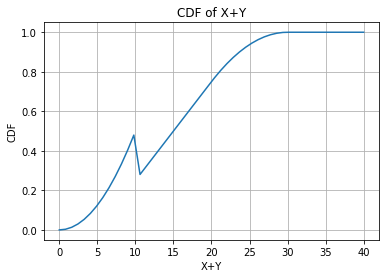
\includegraphics[width=0.5\textwidth]{assignment6cdf.png}
\end{center}
\end{figure}

\end{document}